\documentclass[a4paper, 11pt]{article}
\usepackage[cpp,linenum]{mypackage}
\usepackage{amsmath}
\usepackage{graphicx}
\usepackage{geometry}
\geometry{scale=0.8}
\usepackage{hyperref}
\lstset{language=lisp}


\title{
\normalfont \normalsize
\textsc{School of Data and Computer Science, Sun Yat-sen University} \\ [25pt] %textsc small capital letters
\rule{\textwidth}{0.5pt} \\[0.4cm] % Thin top horizontal rule
\huge  E07 FF Planner \\ % The assignment title
\rule{\textwidth}{2pt} \\[0.5cm] % Thick bottom horizontal rule
\author{17341015 Hongzheng Chen}
\date{\normalsize\today}
}

\begin{document}
\maketitle
\tableofcontents
\newpage

\section{Examples}

\subsection{Spare Tire}
\begin{lstlisting}[title=domain\_spare\_tire.pddl,language=lisp]
(define (domain spare_tire)
  (:requirements :strips :equality:typing)
  (:types physob location)
  (:predicates  (Tire ?x - physob)
		(at ?x - physob ?y - location))

(:action Remove
             :parameters (?x - physob ?y - location)
             :precondition (At ?x ?y)
             :effect (and (not (At ?x ?y)) (At ?x Ground)))

  (:action PutOn
             :parameters (?x - physob)
             :precondition (and (Tire ?x) (At ?x Ground)
                                (not (At Flat Axle)))
             :effect (and (not (At ?x Ground)) (At ?x Axle)))
  (:action LeaveOvernight
             :effect (and (not (At Spare Ground)) (not (At Spare Axle))
                          (not (At Spare Trunk)) (not (At Flat Ground))
                          (not (At Flat Axle)) (not (At Flat Trunk)) ))
 )

\end{lstlisting}
\begin{lstlisting}[title=spare\_tire.pddl,language=lisp]
(define (problem prob)
 (:domain spare_tire)
 (:objects Flat Spare -physob Axle Trunk Ground - location)
 (:init (Tire Flat)(Tire Spare)(At Flat Axle)(At Spare Trunk))
 (:goal (At Spare Axle))
)
\end{lstlisting}
\begin{figure}[H]
  \centering
  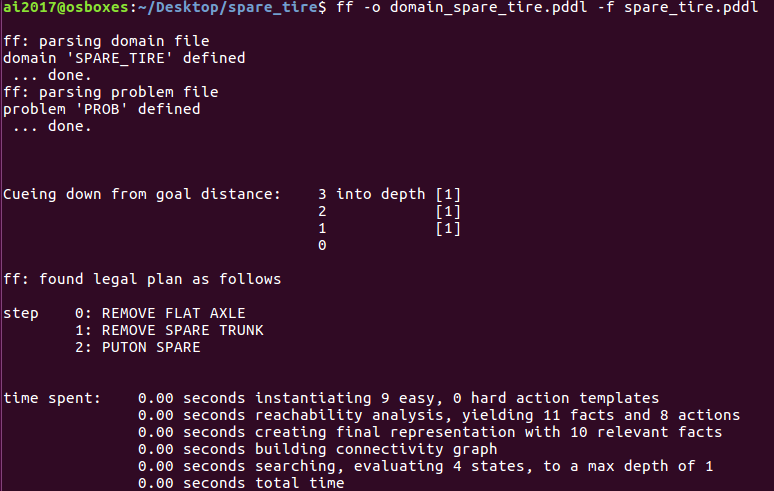
\includegraphics[width=16cm]{fig/spare_tire}
\end{figure}

\subsection{Briefcase World}
Please refer to \texttt{pddl.pdf} at page 2. Please pay More attention to the usages of \texttt{forall} and \texttt{when}.

For more examples, please refer to \texttt{ff-domains.tgz} and \texttt{benchmarksV1.1.zip}. For more usages of FF planner, please refer to the documentation \texttt{pddl.pdf}.
\section{Tasks}

\subsection{8-puzzle}
\begin{figure}[H]
  \centering
  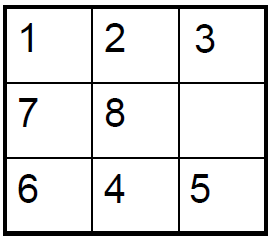
\includegraphics[width=0.4\textwidth]{fig/puzzle}
  \qquad
  \parbox[b]{0.4\textwidth}{Please complete  \texttt{domain\_puzzle.pddl} and \texttt{puzzle.pddl} to solve the 8-puzzle problem.\\}
\end{figure}
\begin{lstlisting}[title=domain\_puzzle.pddl,language=lisp]
(define (domain puzzle)
  (:requirements :strips :equality:typing)
  (:types num loc)
  (:predicates  ())

(:action slide
             :parameters ()
             :precondition ()
             :effect ()
 )
)
\end{lstlisting}
\begin{lstlisting}[title=domain\_puzzle.pddl,language=lisp]
(define (problem prob)
 (:domain puzzle)
 (:objects )
 (:init )
 (:goal ())
)
\end{lstlisting}

\subsection{Blocks World}
\begin{figure}[H]
  \centering
  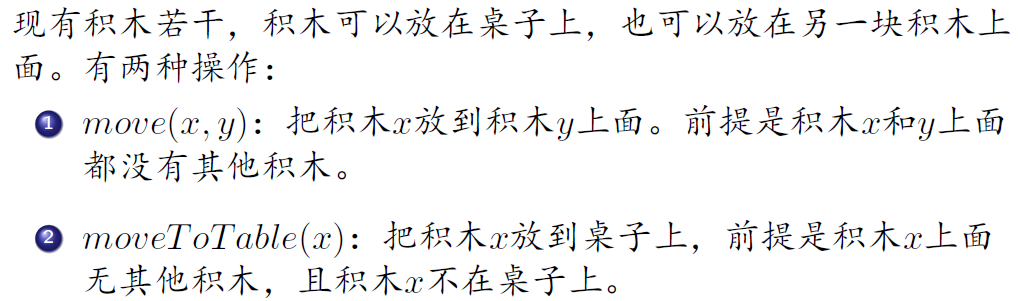
\includegraphics[width=17cm]{fig/blocks}
\end{figure}

Please complete the file \texttt{domain\_blocks.pddl} to solve the blocks world problem. You should know the usages of \texttt{forall} and \texttt{when}.

\begin{lstlisting}[title=domain\_blocks.pddl,frame=single,language=lisp,numbers=left]
(define (domain blocks)
  (:requirements :strips :typing:equality
                 :universal-preconditions
                 :conditional-effects)
  (:types physob)
  (:predicates
  	    (ontable ?x - physob)
            (clear ?x - physob)
	    (on ?x ?y - physob))

  (:action move
             :parameters (?x ?y - physob)
             :precondition ()
             :effect ()
             )

  (:action moveToTable
             :parameters (?x - physob)
             :precondition ()
             :effect ( )
 )
\end{lstlisting}

\begin{lstlisting}[title=blocks.pddl,frame=single,language=lisp,numbers=left]
(define (problem prob)
 (:domain blocks)
 (:objects A B C D E F - physob)
 (:init (clear A)(on A B)(on B C)(ontable C) (ontable D)
  (ontable F)(on E D)(clear E)(clear F)
)
 (:goal  (and (clear F) (on F A) (on A C) (ontable C)(clear E) (on E B)
         (on B D) (ontable D)) )
 )
\end{lstlisting}
Please submit a file named \textsf{E07\_YourNumber.pdf}, and send it to \textsf{ai\_201901@foxmail.com}


\section{Codes and Results}
\subsection{8-Puzzle}
The code below is \verb'domain_puzzle.pddl', which leverages four slide action to describe the movements.
\begin{lstlisting}
  (define (domain puzzle)
  (:requirements :strips :typing)
  (:types num loc)
  (:predicates
      (at-pos ?n ?x ?y)
      (inc ?p ?p1)
      (dec ?p ?p1))
  (:action slide-up
      :parameters (?n ?x ?y ?x1)
      :precondition (and (at-pos ?n ?x ?y) (at-pos n0 ?x1 ?y) (dec ?x ?x1))
      :effect (and (not (at-pos ?n ?x ?y)) (not (at-pos n0 ?x1 ?y))
                  (at-pos ?n ?x1 ?y) (at-pos n0 ?x ?y))
  )
  (:action slide-down
      :parameters (?n ?x ?y ?x1)
      :precondition (and (at-pos ?n ?x ?y) (at-pos n0 ?x1 ?y) (inc ?x ?x1))
      :effect (and (not (at-pos ?n ?x ?y)) (not (at-pos n0 ?x1 ?y))
                  (at-pos ?n ?x1 ?y) (at-pos n0 ?x ?y))
  )
  (:action slide-left
      :parameters (?n ?x ?y ?y1)
      :precondition (and (at-pos ?n ?x ?y) (at-pos n0 ?x ?y1) (dec ?y ?y1))
      :effect (and (not (at-pos ?n ?x ?y)) (not (at-pos n0 ?x ?y1))
                  (at-pos ?n ?x ?y1) (at-pos n0 ?x ?y))
  )
  (:action slide-right
      :parameters (?n ?x ?y ?y1)
      :precondition (and (at-pos ?n ?x ?y) (at-pos n0 ?x ?y1) (inc ?y ?y1))
      :effect (and (not (at-pos ?n ?x ?y)) (not (at-pos n0 ?x ?y1))
                  (at-pos ?n ?x ?y1) (at-pos n0 ?x ?y))
  )
  )
\end{lstlisting}

Below is \verb'puzzle.pddl'.
\begin{lstlisting}
  (define (problem prob)
    (:domain puzzle)
    (:objects n0 n1 n2 n3 n4 n5 n6 n7 n8 p1 p2 p3)
    (:init
        (inc p1 p2)
        (inc p2 p3)
        (dec p3 p2)
        (dec p2 p1)
        (at-pos n1 p1 p1)
        (at-pos n2 p1 p2)
        (at-pos n3 p1 p3)
        (at-pos n7 p2 p1)
        (at-pos n8 p2 p2)
        (at-pos n0 p2 p3)
        (at-pos n6 p3 p1)
        (at-pos n4 p3 p2)
        (at-pos n5 p3 p3)
    )
    (:goal (and
        (at-pos n1 p1 p1)
        (at-pos n2 p1 p2)
        (at-pos n3 p1 p3)
        (at-pos n4 p2 p1)
        (at-pos n5 p2 p2)
        (at-pos n6 p2 p3)
        (at-pos n7 p3 p1)
        (at-pos n8 p3 p2)
        (at-pos n0 p3 p3)
    ))
  )
\end{lstlisting}

The running result is shown below.
For all the actions, please refer to the attached \verb'result1.txt'.
\begin{figure}[H]
  \centering
  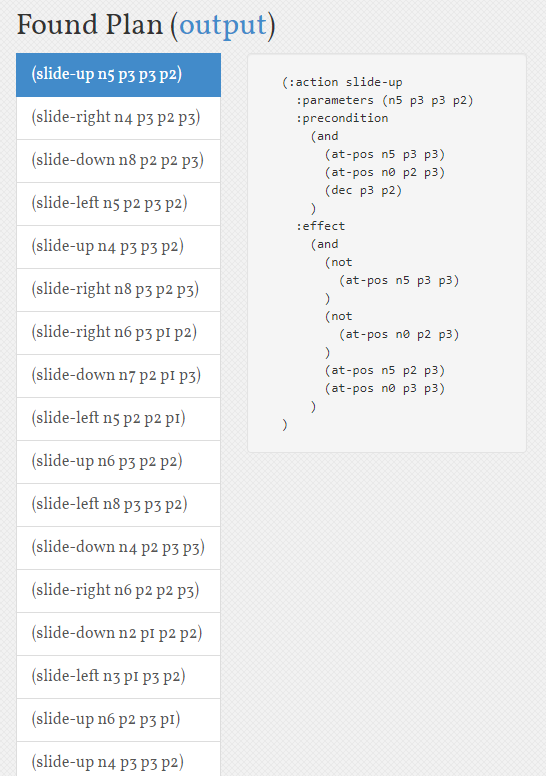
\includegraphics[width=0.5\linewidth]{fig/result1.png}
\end{figure}

\subsection{Block Worlds}
Below is \verb'domain_blocks', which leverages \verb'forall' and \verb'when' grammas to specify the blocks below which to be moved.
\begin{lstlisting}
(define (domain blocks)
(:requirements :strips :typing:equality
               :universal-preconditions
               :conditional-effects)
(:types physob)
(:predicates
  	(ontable ?x - physob)
    (clear ?x - physob)
	(on ?x ?y - physob)
)
(:action move
    :parameters (?x ?y - physob)
    :precondition (and (clear ?x) (clear ?y) (not (= ?x ?y)))
    :effect (and (on ?x ?y) (clear ?x) (not (clear ?y))
                (forall (?z - physob) (when (on ?x ?z) (and (not (on ?x ?z)) (clear ?z))))
                (when (ontable ?x) (not (ontable ?x))))
)
(:action moveToTable
    :parameters (?x - physob)
    :precondition (and (clear ?x) (not (ontable ?x)))
    :effect (and (ontable ?x)
                (forall (?z - physob) (when (on ?x ?z) (and (not (on ?x ?z)) (clear ?z)))))
))
\end{lstlisting}

Below shows \verb'blocks.pddl'.
\begin{lstlisting}
  (define (problem prob)
  (:domain blocks)
  (:objects A B C D E F - physob)
  (:init
      (clear A)
      (on A B)
      (on B C)
      (ontable C)
      (ontable D)
      (ontable F)
      (on E D)
      (clear E)
      (clear F)
  )
  (:goal
      (and (clear F) (on F A) (on A C) (ontable C) (clear E) (on E B)
           (on B D) (ontable D))
  )
  )
\end{lstlisting}

The result is shown below.
\begin{figure}[H]
\centering
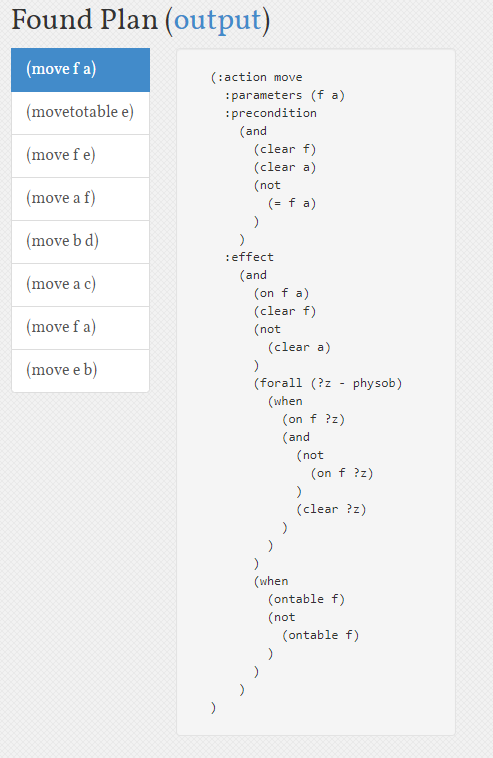
\includegraphics[width=0.5\linewidth]{fig/result2.png}
\end{figure}

\end{document}